\documentclass[a4paper,12pt,twosided]{report}
\usepackage[utf8]{inputenc}
\usepackage{datetime}
\usepackage{url}
\usepackage[pdftex]{graphicx}
\usepackage{amsmath}
\usepackage{mathtools}
\usepackage{epstopdf}
\usepackage{listings}
\usepackage{float}

% Haskell code listing
\usepackage{listings}
\lstloadlanguages{Haskell}
\lstnewenvironment{code}
    {\lstset{}%
      \csname lst@SetFirstLabel\endcsname}
    {\csname lst@SaveFirstLabel\endcsname}
    \lstset{
      basicstyle=\small\ttfamily,
      numbers=left,
      frame=single,
      flexiblecolumns=false,
      basewidth={0.5em,0.45em},
      literate={+}{{$+$}}1 {/}{{$/$}}1 {*}{{$*$}}1 {=}{{$=$}}1
               {>}{{$>$}}1 {<}{{$<$}}1 {\\}{{$\lambda$}}1
               {\\\\}{{\char`\\\char`\\}}1
               {->}{{$\rightarrow$}}2 {>=}{{$\geq$}}2 {<-}{{$\leftarrow$}}2
               {<=}{{$\leq$}}2 {=>}{{$\Rightarrow$}}2 
               {\ .}{{$\circ$}}2 {\ .\ }{{$\circ$}}2
               {>>}{{>>}}2 {>>=}{{>>=}}2
               {|}{{$\mid$}}1               
    }

\newdateformat{monthdate}{\monthname[\THEMONTH] \THEYEAR}

\begin{document}
% Adapted the GU template from word to LaTeX
\begin{titlepage}
\thispagestyle{empty}

\begin{center}
\includegraphics[width=\textwidth]{gulogo.pdf}
\end{center}

\vfill

\begin{flushleft}
{\LARGE Implementing incremental and parallel parsing} \\[0.2cm]
{\large \textit{Master of Science Thesis in Computer Science}}\\[3cm]

{\Huge \textsc{Tobias Olausson}}

\vfill

University of Gothenburg \\
Chalmers University of Technology \\
Department of Computer Science and Engineering \\
Göteborg, Sweden, \monthdate\today
\end{flushleft}

\newpage
\thispagestyle{plain}

\noindent The Author grants to Chalmers University of Technology and University
of Gothenburg  the non-exclusive right to publish the Work electronically and in
a non-commercial purpose make it accessible on the Internet.  The Author
warrants that he is the author to the Work, and warrants that the Work does
not contain text, pictures or other material that violates copyright law.\\

\noindent The Author shall, when transferring the rights of the Work to a third
party (for example a publisher or a company), acknowledge the third party about
this agreement. If the Author has signed a copyright agreement with a third
party regarding the Work, the Author warrants hereby that he has obtained
any necessary permission from this third party to let Chalmers University of
Technology and University of Gothenburg  store the Work electronically and make
it accessible on the Internet. \\[2cm]

\noindent \textbf{Implementing incremental and parallel parsing}\\
\noindent \textsc{Tobias Olausson} \\

\noindent \copyright \textsc{ Tobias Olausson}, \monthdate\today \\

\noindent Examiner: \textsc{Patrik Jansson} \\

\noindent University of Gothenburg \\
Chalmers University of Technology \\
Department of Computer Science and Engineering \\
SE-412 96 Göteborg \\
Sweden \\
Telephone + 46 (0)31-772 1000 \\

\vfill

\noindent Department of Computer Science and Engineering \\
Göteborg, Sweden, \monthdate\today
\end{titlepage}



\begin{abstract}
This is an abstract
\end{abstract}

\tableofcontents

%
% NEW CHAPTER
%

\chapter{Background}

\section{Introduction}
The topic of this thesis is to do \textbf{parsing} in an \textbf{incremental}
fashion that can easily be \textbf{parallelizable}, using a
\textbf{divide-and-conquer approach}. In this section, I will give a brief
explanation of the topics covered, and end with a motivation for why this is
interesting to do in the first place.

\subsection{Divide-and-conquer}
Something in general about them. Maybe mergesort?
Add stuff here from section 2 in parparse paper.

\subsection{Incrementality}
Doing something incrementally means that one does it step by step, and not
longer than neccessary. Not a new idea at all. 

\subsection{Parallelism}
In modern day processors, rather than increasing the clock frequency, efforts are
put into building processors with many cores, being able to run instructions in
parallel. Programmers have for many years written code that runs several
instructions seemingly simultaneous, even on single-core processors. With
multi-core processors this can be done truly in parallel. Since divide-and-conquer
algorithms usually work on several independent sub-problems, they are
well-suited for parallelization. For this to become a reality, however, both the
compiler and the source code must be written in a certain way to permit
parallelization.

\subsection{Parsing}
To parse is a to check if some given input corresponds to a certain language's
grammar, and in this thesis I will use \textbf{context-free grammars} for
programming languages. Many programming errors are syntactical ones, such as
misspelled keywords, missing parenthesis or semicolons and so on. All such
errors are caught in parsing. Parsing will be described in more detail in
section \ref{parsingsection}.

\subsection{Motivation}
In compilers, lexing and parsing are the two first phases. The output of these
is an abstract syntax tree (AST) which is fed to the next phase of the compiler.
But an AST could also provide useful feedback for programmers, already in their
editor, if the code could be lexed and parsed fast enough. With a lexer and
parser that is incremental and that can also be parallelized could real-time
feedback in the form of an AST easily be provided to the programmer. Most
current text editors give syntax feedback based on regular expressions, which
does not yield any information about depth or the surrounding AST.

Something something about connecting to a type-checker.

\section{Lexing}
In compilers, a \textit{lexer} reads input source code and groups the characters
into sequences called \textit{lexemes} so that each lexeme has some meaning in
the language the compiler is built for \cite[p. 5, p. 109]{dragonbook}. The
lexemes are wrapped in \textit{tokens} that denote what function and position
each lexeme has. The tokens are then passed on to the parser for syntactic
analysis.

For a language like C, the code in figure \ref{lexsample} would be valid, and
can serve as an example of how lexing is done.
\begin{figure}[H]
\begin{code}
while(i < 5) {
    i++;
}
\end{code}
\caption{A while loop that would be valid in C}
\label{lexsample}
\end{figure}
A lexer would recognise that \textit{while} is a keyword and place it in its own
token. It would also observe that (, ), \textit{\{} and \textit{\}} are used for
control grouping of code. Furthermore, i is an identifier and 5 is a number, $<$
and ++ are operators and ; denote separation of statements. All of these will be
forwarded as tokens to the parser.

\subsection{LexGen}
As a master's thesis, a generator for incremental divide-and-conquer lexers was
developed in 2013 by Hansson and Hugo \cite{divconqlex}. Since the aim of this
thesis is to write an incremental divide-and-conquer parser, their work is
well-suited as a starting point, and as something to build on. Their lexer
utilised Alex for core lexing routines and relied heavily on the use of arrays
and finger trees, which we will see more of later. 

\section{Context-free grammars}
Context-free grammars are a way to describe formal languages, such as
programming languages. They describe both the alphabet of a language and the
rules for how to combine words in that language.

Formally, a context-free grammar is a 4-tuple: $G = (V, \Sigma, P, S)$
\cite[p.171]{automatabook}. $V$ is a set of non-terminals, or variables. $\Sigma$ is
the set of terminal symbols, describing the content (or alphabet) that can be
written in the language.  $P$ is a set of productions (or rewrite rules) that
constitutes the recursive definition of the language. $S$ is the start symbols,
where $S \in V$. 

The language recognized by a context-free grammar $G$ is denoted $L(G)$ and is
defined as 
\[
L(G) = \{w \in \Sigma^* \ |\  S \xRightarrow[G]{*} w\}
\]
That is, all words in the language that can be derived using the rules from the
grammar and starting from the start symbol \cite[p. 177]{automatabook}.  A
language $L$ is said to be context-free if there is a context-free grammar $G$
that recognizes the language, meaning that $L = L(G)$.

We can exemplify this using a simple made-up language of if-then-else clauses.
The language terminals are \textit{if, then, else} and \textit{true and false}.
There are two variables, \textit{I} (for if) and \textit{R} (for recursive)
described by a total of four productions. The starting symbol is \textit{I} - so
just writing \textit{true} would not be valid for this language. The formal
definition of such a language can be seen in figure \ref{iflang}.

\begin{figure}[H]
\begin{align*}
G &= (V, \Sigma , P, I) \\
V &= \{I,R\} \\
\Sigma &= \{true,false,if,then,else\} \\
I &\rightarrow if\ R\ then\ R\ else\ R \\
R &\rightarrow I \\
R &\rightarrow true \\
R &\rightarrow false
\end{align*}
\caption{Context-free grammar for a recursive if-then-else language}
\label{iflang}
\end{figure}

\subsection{Backus-Naur Form}
TODO: John Backus wrote a paper on this, cite it? See compling-essay.

Context-free grammars are often used to describe the syntax of programming
languages. Such descriptions are often given in a \textbf{labelled Backus-Naur
form}, where each rule is written on the following form:
\[
Label.\ Variable ::= Production 
\]

Just link to BNFC here?

Grammars written in Labelled Backus-Naur Form are also used in the \textbf{BNF
Converter (BNFC)}, a lexer and parser generator tool developed at Chalmers.
Given such a grammar, BNFC generates, among other things, a lexer and a parser,
implemented in one of several languages, for the language described in that
grammar. According to its documentation, usage of BNFC saves approx 90\% of
source code work in writing a compiler front-end. 

\subsection{Chomsky Normal Form}
Chomsky Normal Form (CNF) is a subset of context-free grammars that was first
described by linguist Noam Chomsky. Productions in CNF are restricted to the
following forms:

\begin{figure}[H]
\begin{tabular}{l l l l}
    A & $\rightarrow$ & BC, & A is a variable, B and C are productions \\
    A & $\rightarrow$ & a, & A is a variable, a is a terminal symbol \\
\end{tabular}
\caption{Rules allowed in Chomsky Normal Form}
\end{figure}
Since grammars in CNF are restricted to branches or single terminal symbols,
they are well suited for usage in divide-and-conquer algorithms. There are
several existing algorithms to convert context-free grammars into CNF, so one
does not have to write their grammars in CNF in the first place \cite{langeleiss}.

\section{Parsing}
\label{parsingsection}
The role of the parser is, given a list of tokens, to determine if that those
tokens can be written in that order for a specific language. More precise, and
connecting to the language of a context-free grammar above, the parser is given
a string $w$ and checks if 
\[
w \in \Sigma^*, S \xRightarrow[G]{*} w
\]
that is, to check if the given string can be generated by applying the grammar
rules recursively. There are many different algorithms to do this, most common
are LL(k) and LR(k) parsers that are bottom-up and top-down parsers,
respectively \cite[p.192]{dragonbook}. This project however, will employ neither
technique, but instead use a variant of the CYK algorithm. 

\subsection{CYK algorithm}
The CYK algorithm is named after its inventors Cocke, Younger and Kasami, who
independently created the algorithm in the late 1960s. % TODO: Cite Younger and Kasami

\subsection{Valiant}
0-1-matrices improvement. 
\subsection{Improvement by Bernardy \& Claessen}
Running time analysis. Oracle for lists. 

\section{Dependently typed programming}
In a strictly typed programming language like Haskell, every value has a type
that is enforced. Assigning an integer a floating-point value would not
type-check and therefore would not compile. While this is useful and saves
debugging time, it does not say anything about the contents of the values.

A motivating example often used is implementation of a vector type. Vectors in
this case is a fixed-length list of some type. In a typical Haskell setting we 
may have a type as follows:
\begin{figure}[H]
\begin{code}
data Vec a = Nil | V a Vec

head :: Vec a -> a
head Nil = error "empty vector"
head (V a _) = a
\end{code}
\caption{Vector type and head function}
\end{figure}
This looks good, but it has the inherent problem that any code that tries to
access the head of an empty Vec will compile but result in a runtime error. 

In dependently typed programming, types may contain other types, acting as
values, so that they relate the same way a value relates to its type. While
Haskell is not a dependently typed programming language, there are ways to use
dependent types even in Haskell. For our vector example that would look
something like this:
\begin{figure}[H]
\begin{code}
data Nat = Z | S Nat
data Vec a n where
    Nil :: Vec a Z
    V :: a -> Vec a s -> Vec a (S s)

head :: Vec a (S b) -> a
head Nil = error "empty vector" -- this does not type-check
head (V a _) = a
\end{code}
\caption{Dependently typed vector with head function}
\end{figure}
We created a new type Nat (for natural numbers) to keep track of the size of our
vector. The new Vec type is \textit{dependent} on the Nat type, while still
holding values of some type \texttt{a}. What this code does not permit, however,
is the Nil case for head. Because the type of head requires the Vec to be
non-nil (with (S b) in its type signature) there is no need to check for a Nil
vector here. In fact, the compiler will not pass the above code, as indicated by
the comment, since the first case in head does not type check. The main
advantage of this vector type is that any code that uses head and passes
type-checking will be guaranteed to never encounter an empty vector.  This way,
even more bugs are caught at compile-time.

%
% NEW CHAPTER
%

\chapter{Implementation}
Before going into details about the implementation of this parser, there are a
couple of libraries and programming techniques one has to be familiar with
before moving forward. I will first describe those, and then move on to describe
changes to the lexer I inherited, and the implementation of the parser.

\section{Finger trees}
A finger tree is a finite data structure with logarithmic time access and
concatenation. The finger tree is similar to a general binary tree, where each
branch has a couple of \textit{fingers} (values) so that adding a new value does
not neccessarily add a new branch to the tree. The tree structure makes the data
structure suitable for a divide-and-conquer algorithm. TODO: Referens till paper
om finger trees

A Haskell implementation suitable for everyday needs exists in the
\texttt{Data.Sequence} package, and a more general structure is available in the
\texttt{Data.FingerTree} package. The more general one is the one that will be
used for this project, and is the one that was used for the LexGen project.

\subsection{Measuring and Monoids}
Two specific features in the general FingerTree data type are monoids and
measuring. These are fundamental to the parser, so we will look more deeply into
them here.

A \textit{monoid} is a mathematical object with an identity element and an
associative operation. In Haskell, this is provided by writing instances of this
type class:
\begin{figure}[H]
TODO: Src-referens
\begin{code}
class Monoid a where
    -- Identity of mappend
    mempty  :: a
    -- An associative operation
    mappend :: a -> a -> a
\end{code}
\caption{The Monoid type class}
\end{figure}
This means that anything that is a Monoid has an identity element (that can be
accessed with \textit{mempty}) and an associative operation to append monoids
together (\textit{mappend}). A simple list example illustrates this:
\begin{figure}[H]
\begin{code}
instance Monoid [a] where
    mempty = []
    mappend = (++)
\end{code}
\caption{Monoid instance for lists}
\end{figure}
TODO: Say something more about Monoids?

The FingerTree type has a notion of being able to \textit{measure} its elements.
In this case, to measure means to have a function that, given an element of the
type the FingerTree contains, yields a value of some type -- the measure of that
element. Furthermore, any type that the elements can be measured to has to be a
monoid. The existance of a measured instance is ensured by the FingerTree API. 
\begin{figure}[H]
TODO: src-referens
\begin{code}
-- Things that can be measured
class Monoid v => Measured v a | a -> v where
    measure :: a -> v

-- FingerTrees are parametrized on both v (measures) and a (values)
data FingerTree v a

-- Create an empty finger tree
empty :: Measured v a => FingerTree v a
\end{code}
\caption{Measuring and the FingerTree type}
\end{figure}
This means that, in order to use the FingerTree, one need to fulfil a few
criteria first. Let's say you want to have a FingerTree of Strings and that the
measure should be the (combined) length of the Strings, then your type would be
\texttt{FingerTree Int String}. For that to work, you first need to be able to
convert between Strings and Int, by writing an instance of Measured for String
Int. This would typically just be the length function. However, for that to work
you need a Monoid instance for Ints. Perhaps it would look something like this:

\begin{figure}[H]
\begin{code}
type MyTree = FingerTree Int String
instance Measured String Int where
    measure = length
instance Monoid Int where
    mempty = 0
    mappend = (+)
\end{code}
\caption{One possible measure from String to Int}
\end{figure}
It should be noted however, that since instances cannot be hided, writing a
general Monoid instance for Ints over addition is perhaps not the best idea.
Wrapper types with instances over addition and multiplication are available in
the \texttt{Data.Monoid} library.

\section{Lexing}
For lexing code into tokens, the results from the LexGen project was used.
However, some modifications had to be done to LexGen in order to be easily
generated from BNFC as an Alex file. One large change was done to the lexing
code, however, which is due to the fact that not only the lexer, but also the
parser, should work incrementally. In the LexGen code, the output structure is a
\texttt{Sequence} of tokens. Since \texttt{Sequence} is a less general
implementation of finger trees, they cannot be measured, and is therefore not as
suitable to use in an incremental setting. Hence, instead of outputting tokens
as a \texttt{Sequence}, the code was changed to output as another
\texttt{FingerTree}, from which the tokens could then be measured (see section
\ref{pipeline} below).
TODO: Code here?

\section{Parsing}
TODO: Move this part down? Duplicate in BNFC
TODO: An illustration here perhaps?

Observing that the lexer could easily be generated from BNFC, it was natural to
plug it in, and given that, the parser code is so general that it can also be
generated from any LBNF grammar.
\subsection{BNFC}
There was an existing reference implementation in BNFC for the optimisation to
Valiant's algorithm, that could be accessed using the \texttt{--cnf} option.
That option generated large tables needed for combining different tokens. Since
the this project is similar to the reference implementation, it was natural to
generate the new parser by using a new option.

For the Haskell backend, BNFC uses Alex as a lexer, as did LexGen, so it was
easy to use the LexGen core and have BNFC and Alex generate the DFA needed for
the lexer to work. 

\subsection{Pipeline of measures}
\label{pipeline}
TODO: Clarify that ONE char does not become the whole AST. Tree structure!
TODO: Paste code with Measured constraints on the Measured instance!

Using the \texttt{FingerTree} type, the lexer could use that data type to
measure characters into an intermediate type for lexing. That intermediate
\texttt{FingerTree} could then in turn be measured to the type used for parsing.
\begin{figure}[H]
Picture here as soon as its pushed to the repo.
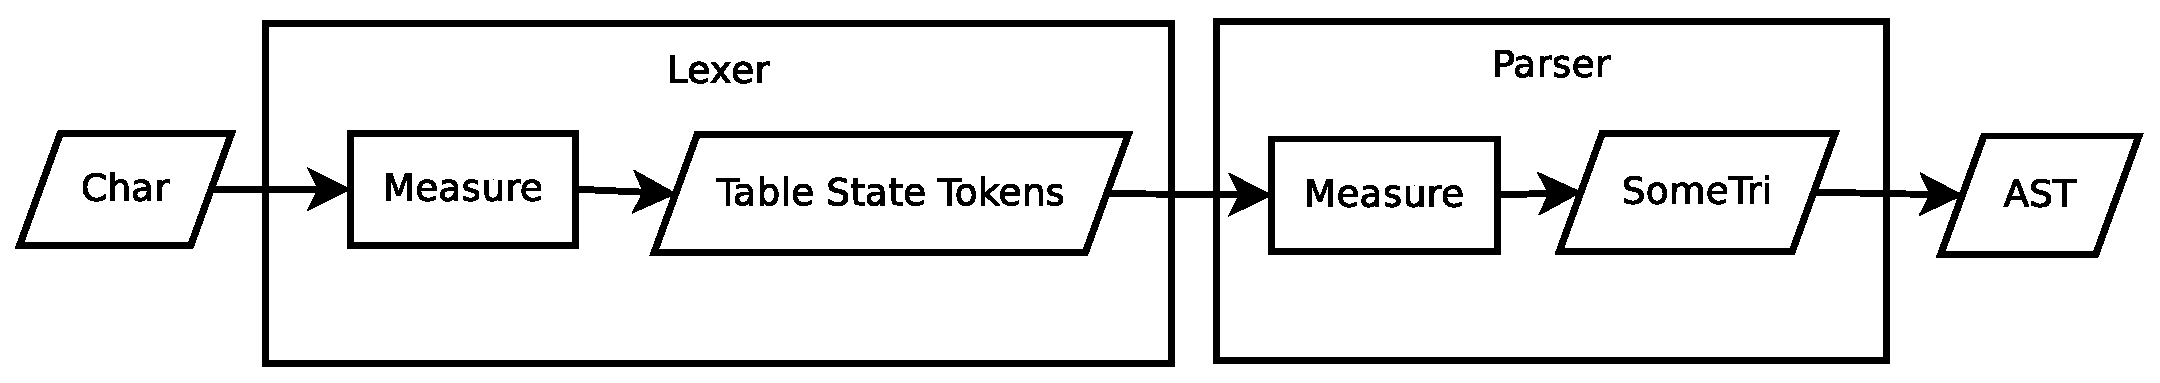
\includegraphics[width=\textwidth]{pipeline.eps}
\caption{Diagram of measuring pipeline}
\end{figure}
Looking at simple testing code shows easily how the data progresses through the
pipeline. \texttt{stateToTree} is an auxiliary function extracting a
\texttt{FingerTree} from the internal lexer state.

\begin{figure}[H]
\begin{code}
test :: FilePath -> IO (SomeTri [(CATEGORY,Any)])
test filename = do
    file <- readFile filename
    let mes = measure $ makeTree file
        tri = measure $ stateToTree mes
    return (results tri)
\end{code} 
\caption{Code showing the measuring pipeline}
\end{figure}
The \texttt{Measured} instance for the lexer was written as part of the LexGen
project, and was only slightly modified to fit the parser. The \texttt{Measured}
instance for the parser is far more interesting, though. We can se how it works
in figure \ref{parsemeasure}

\begin{figure}[H]
TODO: A figure
\begin{code}
instance Measured (SomeTri [(CATEGORY,Any)]) IntToken where
    -- Note: place the token just above the diagonal
    measure tok = T (bin' Leaf' Leaf') (q True :/: q False)
      where q b = quad zero (t b) zero zero
            select b = if b then leftOf else rightOf
            t b = case intToToken tok of
                Nothing    -> Zero
                Just token -> One $ select b $ tokenToCats b token

\end{code}
\caption{\label{parsemeasure} Measure from token to upper-triangular matrix}
\end{figure}
We create a 2x2 matrix, and place the token in the upper-right corner -- just
above the diagonal. 

TODO: The Monoid instance here as well.

\subsection{Dependently typed programming with charts}
The \texttt{SomeTri} type is the type representing upper-triangular matrices in
the code. Merging these matrices is the central to the parsing process. Merging
employs extensions to the code used as a reference to the paper by Bernardy and
Claessen. The matrix code, available from BNFC as a library called
\texttt{Data.Matrix.Quad} is written in a dependently typed fashion.
% TODO: Referens till repo-forken.

First, the matrix type \texttt{Mat} is dependent on another type,
\texttt{Shape}, that describes the shape of a matrix as a binary tree.

\begin{figure}[H]
\begin{code}
data Shape = Bin Shape Shape | Leaf

data Mat :: Shape -> Shape -> * -> * where
  Quad :: !(Mat x1 y1 a) -> !(Mat x2 y1 a) ->
          !(Mat x1 y2 a) -> !(Mat x2 y2 a) ->
          Mat (Bin x1 x2) (Bin y1 y2) a
  Zero :: Mat x y a
  One :: !a -> Mat Leaf Leaf a
  Row :: Mat x1 Leaf a -> Mat x2 Leaf a -> Mat (Bin x1 x2) Leaf a
  Col :: Mat Leaf y1 a -> Mat Leaf y2 a -> Mat Leaf (Bin y1 y2) a
\end{code}
\caption{The \texttt{Mat} type with its dependent \texttt{Shape} type. Note that
shapes are used both for x-axis and y-axis size}
\end{figure}
In a setting without using FingerTrees and Monoids, such as the reference
implementation from the paper, it is possible to merge matrices using a single
element as glue. Such an approach simplifies the merging a lot, since elements
are placed just above the diagonal and that means a single element can fill the
small void in the merged matrix, as illustrated in figure \label{mergein}.

\begin{figure}[H]
Till vänster, mergein MED element
Till höger, merge UTAN element
\caption{\label{mergein}\texttt{merge} with and without a single element as glue}

\end{figure}
Because of the absence of an extra element, the existing mergein function could
not be used, but a merge function had to be implemented. Observing that the V
function from Valiant's algorithm that computes the uppermost matrix when
merging uses a single element, we want to imitate that behaviour. The solution:
chop off the first row in the second argument, and recompute all but the
leftmost elements when applying V. 

TODO: Figur här som förklarar chop-grejen.

\begin{figure}[H]
\begin{code}
merge :: Bool -> SomeTri a -> SomeTri a -> SomeTri a
merge p (T y l) (T x r) = chopShape x $ \chopper x' ->
    let (rTopL, rL') = chopFirst chopper (leftOf r)
        (rTopR, rR') = chopFirst chopper (rightOf r)
        cdp = closeDisjointP p (leftOf l) 
                (mkLast' y $ sequenceA (rTopL :/: rTopR)) rR'
    in T (bin' y x') (quad' l cdp zero (rL' :/: rR'))
\end{code}
\caption{merge without middle element}
\label{merge}
\end{figure}
Looking at the code in figure \ref{merge}, there are a few things to note before
we look more deeply into this. First, \texttt{chopShape} operates on the x-axis
shape in the matrix, returning a continuation containing \texttt{chopper} and a
new x-shape. \texttt{chopper} is of type \texttt{ChopFirst}, which provides an
easy way to pattern match on the x-shape of a \texttt{Mat}, as we can se if we
look at \texttt{chopFirst}, which utilises this.

\begin{figure}[H]
\begin{code}
data ChopFirst x x' where
  Stop :: ChopFirst (Bin Leaf x) x
  Continue :: ChopFirst x x' -> ChopFirst (Bin x x0) (Bin x' x0)

chopFirst :: ChopFirst x x' -> Mat x x a  
                            -> (Mat x' Leaf a, Mat x' x' a)
chopFirst _ Zero = (Zero,Zero)
chopFirst Stop (Quad a b c d) = (b,d)
chopFirst (Continue q) (Quad a b c d) =
  let  (e, a') = chopFirst q a
       (b',f)  = chopFirstRow q b
  in (row e f,quad a' b' zero d)
\end{code}
\caption{\label{chopfirst} ChopFirst type and corresponding function}
\end{figure}

Note that chopFirst, as seen in figure \ref{chopfirst} does not match the
\texttt{Col}, \texttt{Row} or \texttt{One} constructors. For the \texttt{One}
case it is quite obvious because we cannot chop a 1x1 matrix. For the other two,
this is due to the type of \texttt{chopFirst}, where the input is a square
matrix: \texttt{Mat x x a}. Because both \texttt{Col} and \texttt{Row} cannot be
square (unless they're 1x1, in which case the \texttt{One} construct should be
used instead, which cannot be chopped anyway), there is no need to check for
them, and actually writing those cases would trigger a type error when
compiling.

Finally, before calling \texttt{closeDisjointP} (which represents the V function
from Valiant's algorithm), we throw away all but the lower leftmost value, using
\texttt{mkLast'}. The resulting new matrix is a quad, where the left matrix is
left untouched, the right is chopped and a new matrix that serves as top-right
is computed. As usual, all values below the diagonal are zero.

TODO: Explain the recomputation.
TODO: Figur, typ fyrfältare. Left, CDP, Zero, ChoppedRight.

\subsection{Oracle and unsafePerformIO}
The use of an oracle presented a bit of a problem in implementing a monoid
instance for the parser, for the simple reason that it is very hard to simply
pick a bool at random in Haskell without it being always \texttt{True} or always
\texttt{False}. The call to \texttt{merge} in \texttt{mappend} illustrates this
clearly:
\begin{figure}[H]
\begin{code}
instance Monoid (SomeTri a) where
    t0 `mappend` t1 = merge True t0 t1
\end{code}
\caption{Parser Monoid instance before random oracle}
\end{figure}
The call to \texttt{merge} requires a \texttt{Bool} acting as the oracle as an
argument. Since a Monoid has no context outside its own type, it is hard, if not
impossible, to generate a Bool using only the SomeTri type. One could argue for
creating a newtype wrapper around a tuple of a SomeTri and a StdGen, used to
generate the bool at each step, but that only moves the problem to the mempty
call, where a fresh StdGen would have to be picked at each instance.

The solution to this problem came in the form of a call to unsafePerformIO.
While this is controversial, it was also not completely obvious to implement. If
an unsafe call to randomIO was made separately from the merge call, this call
would be evaluated only once, rendering the solution useless. The trick here was
to put the whole call inside an unsafe wrapper, so that the call to merge, and
with that the call to randomIO, became dependent on the input.
\begin{figure}[H]
\begin{code}
instance Monoid (SomeTri a) where
    t0 `mappend` t1 = unsafePerformIO $ do
      b <- randomIO
      return $ merge b t0 t1
\end{code}
\caption{Parser Monoid instance with oracle}
\end{figure}
Now usually, for \texttt{unsafePerformIO} to be safe one should make sure that
the call is free from side effects and \textit{independent of its environment}.
\cite{unsafeHackage}. Since none of those two requirements are fulfilled here
this calls for discussion. In general, one does not want a call to
unsafePerformIO to be evaluated more than once -- but in this case this is a
requirement for the code to behave as expected, and that's why it is indeed
dependent on its environment. The only side effect in this snippet is the use of
the global random number generator and that should not affect any other part of
the program, and can thus be considered safe.

%
% NEW CHAPTER
%

\chapter{Results}

\section{Final product}
\subsection{Testing}

\section{Measurements}
How fast is it? What is the complexity?

%
% NEW CHAPTER
%
\chapter{Discussion}

\section{Pitfalls}
Look through the LOG to remember whatever happened. Describe sort of chronologically?

\subsection{Too many result branches}
Describe the reason for this, with the merge stuff.

\subsection{Position information}
* Tuple of monoids?
* RingP instance?
* Newtype for tuples?

\section{Future work}

%
% BIBLIOGRAPHY
%

% TODO: Decide on some style here
\bibliographystyle{alpha}
\bibliography{bibliography}

%
% ANY APPENDICES HERE
%

\end{document}
